\documentclass[1p]{elsarticle_modified}
%\bibliographystyle{elsarticle-num}

%\usepackage[colorlinks]{hyperref}
%\usepackage{abbrmath_seonhwa} %\Abb, \Ascr, \Acal ,\Abf, \Afrak
\usepackage{amsfonts}
\usepackage{amssymb}
\usepackage{amsmath}
\usepackage{amsthm}
\usepackage{scalefnt}
\usepackage{amsbsy}
\usepackage{kotex}
\usepackage{caption}
\usepackage{subfig}
\usepackage{color}
\usepackage{graphicx}
\usepackage{xcolor} %% white, black, red, green, blue, cyan, magenta, yellow
\usepackage{float}
\usepackage{setspace}
\usepackage{hyperref}

\usepackage{tikz}
\usetikzlibrary{arrows}

\usepackage{multirow}
\usepackage{array} % fixed length table
\usepackage{hhline}

%%%%%%%%%%%%%%%%%%%%%
\makeatletter
\renewcommand*\env@matrix[1][\arraystretch]{%
	\edef\arraystretch{#1}%
	\hskip -\arraycolsep
	\let\@ifnextchar\new@ifnextchar
	\array{*\c@MaxMatrixCols c}}
\makeatother %https://tex.stackexchange.com/questions/14071/how-can-i-increase-the-line-spacing-in-a-matrix
%%%%%%%%%%%%%%%

\usepackage[normalem]{ulem}

\newcommand{\msout}[1]{\ifmmode\text{\sout{\ensuremath{#1}}}\else\sout{#1}\fi}
%SOURCE: \msout is \stkout macro in https://tex.stackexchange.com/questions/20609/strikeout-in-math-mode

\newcommand{\cancel}[1]{
	\ifmmode
	{\color{red}\msout{#1}}
	\else
	{\color{red}\sout{#1}}
	\fi
}

\newcommand{\add}[1]{
	{\color{blue}\uwave{#1}}
}

\newcommand{\replace}[2]{
	\ifmmode
	{\color{red}\msout{#1}}{\color{blue}\uwave{#2}}
	\else
	{\color{red}\sout{#1}}{\color{blue}\uwave{#2}}
	\fi
}

\newcommand{\Sol}{\mathcal{S}} %segment
\newcommand{\D}{D} %diagram
\newcommand{\A}{\mathcal{A}} %arc


%%%%%%%%%%%%%%%%%%%%%%%%%%%%%5 test

\def\sl{\operatorname{\textup{SL}}(2,\Cbb)}
\def\psl{\operatorname{\textup{PSL}}(2,\Cbb)}
\def\quan{\mkern 1mu \triangleright \mkern 1mu}

\theoremstyle{definition}
\newtheorem{thm}{Theorem}[section]
\newtheorem{prop}[thm]{Proposition}
\newtheorem{lem}[thm]{Lemma}
\newtheorem{ques}[thm]{Question}
\newtheorem{cor}[thm]{Corollary}
\newtheorem{defn}[thm]{Definition}
\newtheorem{exam}[thm]{Example}
\newtheorem{rmk}[thm]{Remark}
\newtheorem{alg}[thm]{Algorithm}

\newcommand{\I}{\sqrt{-1}}
\begin{document}

%\begin{frontmatter}
%
%\title{Boundary parabolic representations of knots up to 8 crossings}
%
%%% Group authors per affiliation:
%\author{Yunhi Cho} 
%\address{Department of Mathematics, University of Seoul, Seoul, Korea}
%\ead{yhcho@uos.ac.kr}
%
%
%\author{Seonhwa Kim} %\fnref{s_kim}}
%\address{Center for Geometry and Physics, Institute for Basic Science, Pohang, 37673, Korea}
%\ead{ryeona17@ibs.re.kr}
%
%\author{Hyuk Kim}
%\address{Department of Mathematical Sciences, Seoul National University, Seoul 08826, Korea}
%\ead{hyukkim@snu.ac.kr}
%
%\author{Seokbeom Yoon}
%\address{Department of Mathematical Sciences, Seoul National University, Seoul, 08826,  Korea}
%\ead{sbyoon15@snu.ac.kr}
%
%\begin{abstract}
%We find all boundary parabolic representation of knots up to 8 crossings.
%
%\end{abstract}
%\begin{keyword}
%    \MSC[2010] 57M25 
%\end{keyword}
%
%\end{frontmatter}

%\linenumbers
%\tableofcontents
%
\newcommand\colored[1]{\textcolor{white}{\rule[-0.35ex]{0.8em}{1.4ex}}\kern-0.8em\color{red} #1}%
%\newcommand\colored[1]{\textcolor{white}{ #1}\kern-2.17ex	\textcolor{white}{ #1}\kern-1.81ex	\textcolor{white}{ #1}\kern-2.15ex\color{red}#1	}

{\Large $\underline{11a_{67}~(K11a_{67})}$}

\setlength{\tabcolsep}{10pt}
\renewcommand{\arraystretch}{1.6}
\vspace{1cm}\begin{tabular}{m{100pt}>{\centering\arraybackslash}m{274pt}}
\multirow{5}{120pt}{
	\centering
	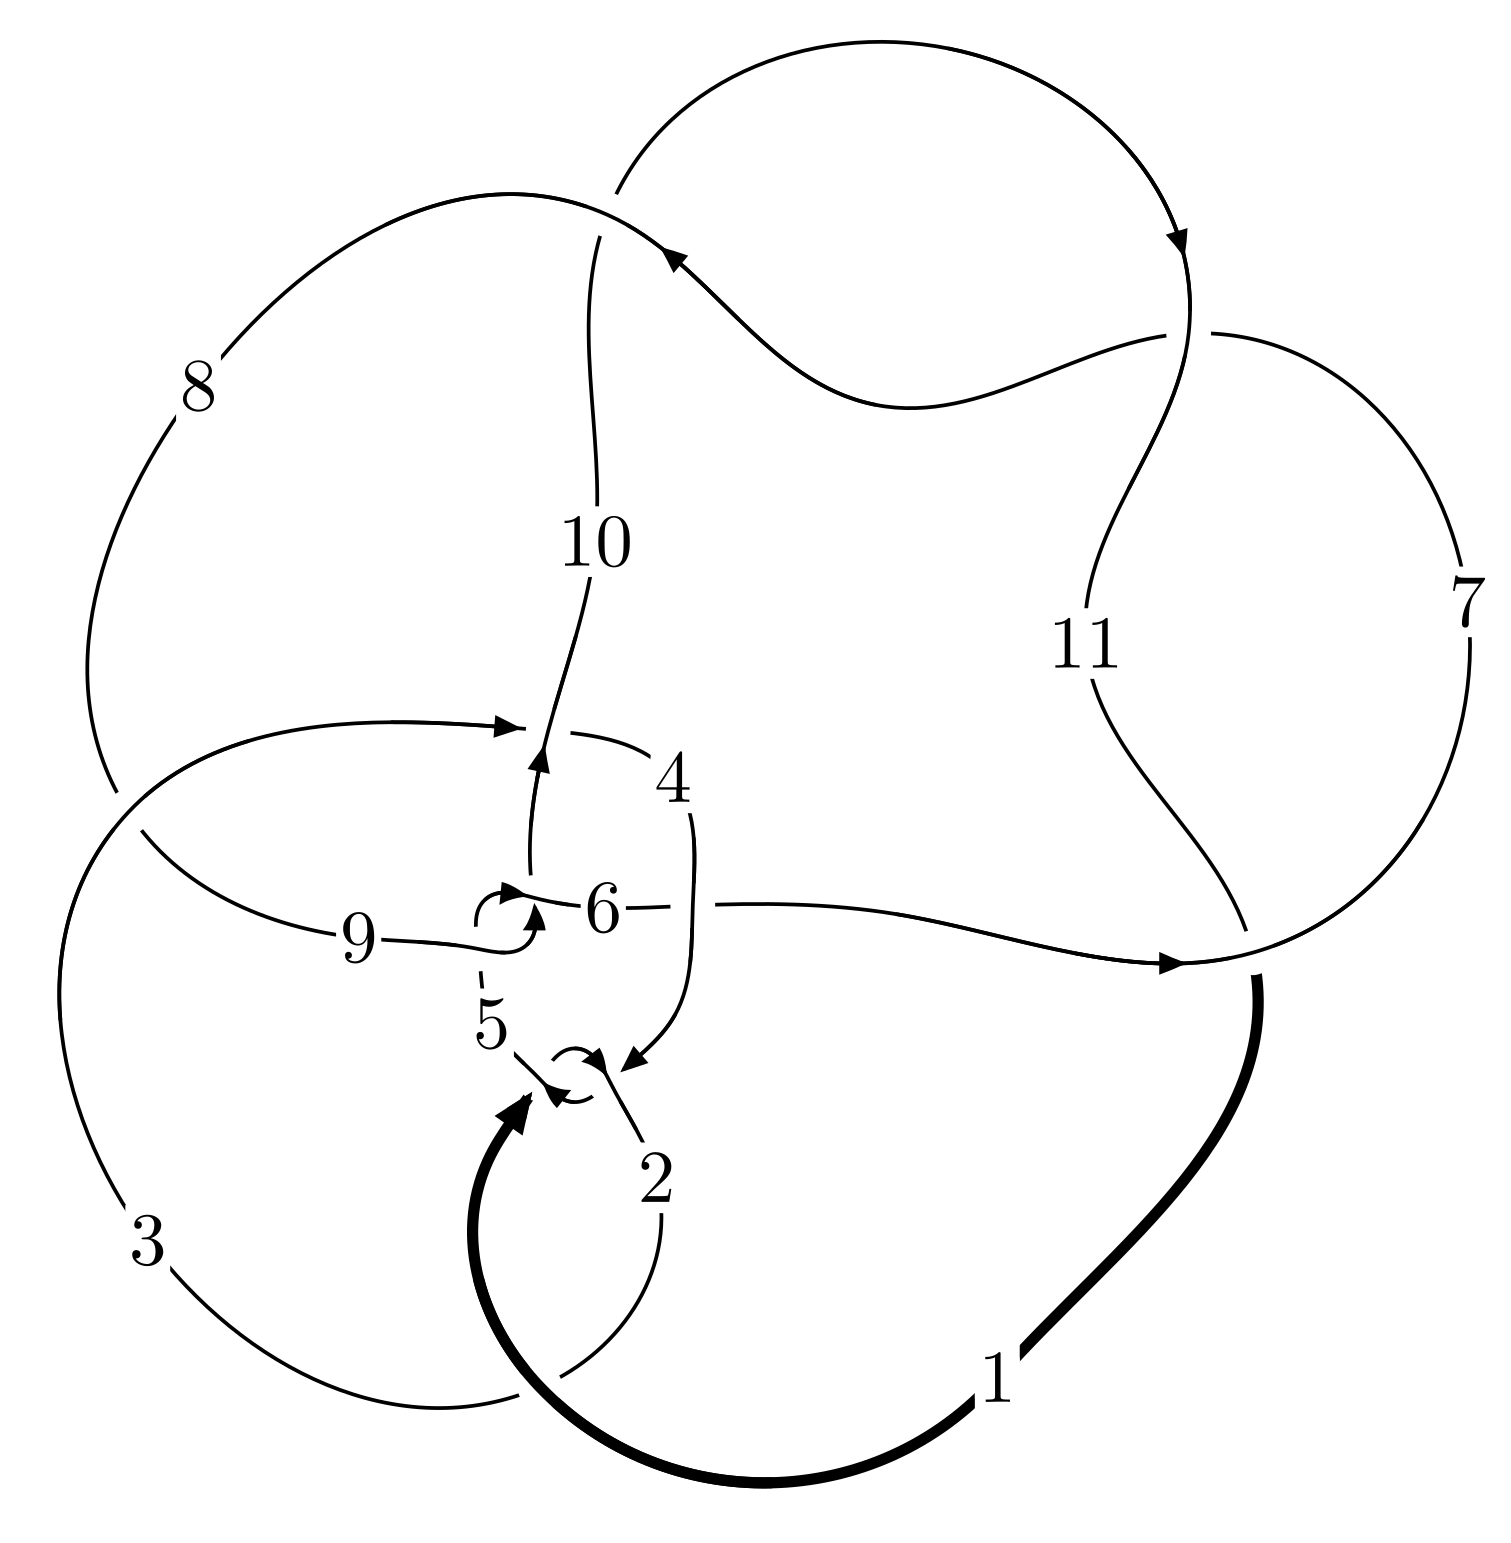
\includegraphics[width=112pt]{../../../GIT/diagram.site/Diagrams/png/316_11a_67.png}\\
\ \ \ A knot diagram\footnotemark}&
\allowdisplaybreaks
\textbf{Linearized knot diagam} \\
\cline{2-2}
 &
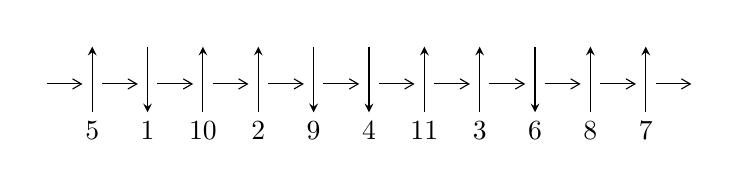
\begin{tikzpicture}[x=20pt, y=17pt]
	% nodes
	\node (C0) at (0, 0) {};
	\node (C1) at (1, 0) {};
	\node (C1U) at (1, +1) {};
	\node (C1D) at (1, -1) {5};

	\node (C2) at (2, 0) {};
	\node (C2U) at (2, +1) {};
	\node (C2D) at (2, -1) {1};

	\node (C3) at (3, 0) {};
	\node (C3U) at (3, +1) {};
	\node (C3D) at (3, -1) {10};

	\node (C4) at (4, 0) {};
	\node (C4U) at (4, +1) {};
	\node (C4D) at (4, -1) {2};

	\node (C5) at (5, 0) {};
	\node (C5U) at (5, +1) {};
	\node (C5D) at (5, -1) {9};

	\node (C6) at (6, 0) {};
	\node (C6U) at (6, +1) {};
	\node (C6D) at (6, -1) {4};

	\node (C7) at (7, 0) {};
	\node (C7U) at (7, +1) {};
	\node (C7D) at (7, -1) {11};

	\node (C8) at (8, 0) {};
	\node (C8U) at (8, +1) {};
	\node (C8D) at (8, -1) {3};

	\node (C9) at (9, 0) {};
	\node (C9U) at (9, +1) {};
	\node (C9D) at (9, -1) {6};

	\node (C10) at (10, 0) {};
	\node (C10U) at (10, +1) {};
	\node (C10D) at (10, -1) {8};

	\node (C11) at (11, 0) {};
	\node (C11U) at (11, +1) {};
	\node (C11D) at (11, -1) {7};
	\node (C12) at (12, 0) {};

	% arrows
	\draw[->,>={angle 60}]
	(C0) edge (C1) (C1) edge (C2) (C2) edge (C3) (C3) edge (C4) (C4) edge (C5) (C5) edge (C6) (C6) edge (C7) (C7) edge (C8) (C8) edge (C9) (C9) edge (C10) (C10) edge (C11) (C11) edge (C12) ;	\draw[->,>=stealth]
	(C1D) edge (C1U) (C2U) edge (C2D) (C3D) edge (C3U) (C4D) edge (C4U) (C5U) edge (C5D) (C6U) edge (C6D) (C7D) edge (C7U) (C8D) edge (C8U) (C9U) edge (C9D) (C10D) edge (C10U) (C11D) edge (C11U) ;
	\end{tikzpicture} \\
\hhline{~~} \\& 
\textbf{Solving Sequence} \\ \cline{2-2} 
 &
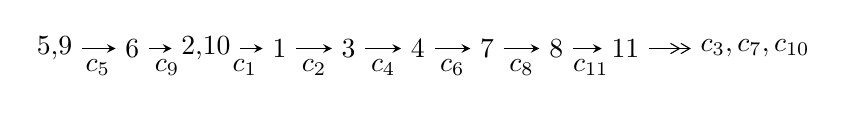
\begin{tikzpicture}[x=25pt, y=7pt]
	% node
	\node (A0) at (-1/8, 0) {5,9};
	\node (A1) at (1, 0) {6};
	\node (A2) at (33/16, 0) {2,10};
	\node (A3) at (25/8, 0) {1};
	\node (A4) at (33/8, 0) {3};
	\node (A5) at (41/8, 0) {4};
	\node (A6) at (49/8, 0) {7};
	\node (A7) at (57/8, 0) {8};
	\node (A8) at (65/8, 0) {11};
	\node (C1) at (1/2, -1) {$c_{5}$};
	\node (C2) at (3/2, -1) {$c_{9}$};
	\node (C3) at (21/8, -1) {$c_{1}$};
	\node (C4) at (29/8, -1) {$c_{2}$};
	\node (C5) at (37/8, -1) {$c_{4}$};
	\node (C6) at (45/8, -1) {$c_{6}$};
	\node (C7) at (53/8, -1) {$c_{8}$};
	\node (C8) at (61/8, -1) {$c_{11}$};
	\node (A9) at (10, 0) {$c_{3},c_{7},c_{10}$};

	% edge
	\draw[->,>=stealth]	
	(A0) edge (A1) (A1) edge (A2) (A2) edge (A3) (A3) edge (A4) (A4) edge (A5) (A5) edge (A6) (A6) edge (A7) (A7) edge (A8) ;
	\draw[->>,>={angle 60}]	
	(A8) edge (A9);
\end{tikzpicture} \\ 

\end{tabular} \\

\footnotetext{
The image of knot diagram is generated by the software ``\textbf{Draw programme}" developed by Andrew Bartholomew(\url{http://www.layer8.co.uk/maths/draw/index.htm\#Running-draw}), where we modified some parts for our purpose(\url{https://github.com/CATsTAILs/LinksPainter}).
}\phantom \\ \newline 
\centering \textbf{Ideals for irreducible components\footnotemark of $X_{\text{par}}$} 
 
\begin{align*}
I^u_{1}&=\langle 
7.57965\times10^{100} u^{65}+1.68003\times10^{101} u^{64}+\cdots+6.92347\times10^{99} b+9.20330\times10^{100},\\
\phantom{I^u_{1}}&\phantom{= \langle  }-2.47059\times10^{101} u^{65}-5.69947\times10^{101} u^{64}+\cdots+2.07704\times10^{100} a-3.70163\times10^{101},\\
\phantom{I^u_{1}}&\phantom{= \langle  }u^{66}+3 u^{65}+\cdots+3 u+1\rangle \\
I^u_{2}&=\langle 
b+u-1,\;3 a+2 u+2,\;u^2- u+1\rangle \\
I^u_{3}&=\langle 
b- u,\;3 a- u+2,\;u^2- u+1\rangle \\
\\
\end{align*}
\raggedright * 3 irreducible components of $\dim_{\mathbb{C}}=0$, with total 70 representations.\\
\footnotetext{All coefficients of polynomials are rational numbers. But the coefficients are sometimes approximated in decimal forms when there is not enough margin.}
\newpage
\renewcommand{\arraystretch}{1}
\centering \section*{I. $I^u_{1}= \langle 7.58\times10^{100} u^{65}+1.68\times10^{101} u^{64}+\cdots+6.92\times10^{99} b+9.20\times10^{100},\;-2.47\times10^{101} u^{65}-5.70\times10^{101} u^{64}+\cdots+2.08\times10^{100} a-3.70\times10^{101},\;u^{66}+3 u^{65}+\cdots+3 u+1 \rangle$}
\flushleft \textbf{(i) Arc colorings}\\
\begin{tabular}{m{7pt} m{180pt} m{7pt} m{180pt} }
\flushright $a_{5}=$&$\begin{pmatrix}1\\0\end{pmatrix}$ \\
\flushright $a_{9}=$&$\begin{pmatrix}0\\u\end{pmatrix}$ \\
\flushright $a_{6}=$&$\begin{pmatrix}1\\u^2\end{pmatrix}$ \\
\flushright $a_{2}=$&$\begin{pmatrix}11.8948 u^{65}+27.4403 u^{64}+\cdots+27.6224 u+17.8216\\-10.9478 u^{65}-24.2657 u^{64}+\cdots-22.9293 u-13.2929\end{pmatrix}$ \\
\flushright $a_{10}=$&$\begin{pmatrix}- u\\- u^3+u\end{pmatrix}$ \\
\flushright $a_{1}=$&$\begin{pmatrix}22.8425 u^{65}+51.7060 u^{64}+\cdots+50.5518 u+31.1145\\-10.9478 u^{65}-24.2657 u^{64}+\cdots-22.9293 u-13.2929\end{pmatrix}$ \\
\flushright $a_{3}=$&$\begin{pmatrix}6.57681 u^{65}+15.6596 u^{64}+\cdots+17.0862 u+11.0579\\-12.8649 u^{65}-27.9088 u^{64}+\cdots-26.2360 u-15.7081\end{pmatrix}$ \\
\flushright $a_{4}=$&$\begin{pmatrix}0.307059 u^{65}+1.87504 u^{64}+\cdots+3.31189 u+3.66520\\-10.3782 u^{65}-22.8004 u^{64}+\cdots-21.2660 u-13.3401\end{pmatrix}$ \\
\flushright $a_{7}=$&$\begin{pmatrix}-11.0251 u^{65}-25.7638 u^{64}+\cdots-23.1138 u-17.5999\\15.7432 u^{65}+36.3559 u^{64}+\cdots+35.5916 u+21.6869\end{pmatrix}$ \\
\flushright $a_{8}=$&$\begin{pmatrix}9.82325 u^{65}+23.5692 u^{64}+\cdots+22.4882 u+14.6165\\-11.2402 u^{65}-24.5385 u^{64}+\cdots-20.0450 u-13.5642\end{pmatrix}$ \\
\flushright $a_{11}=$&$\begin{pmatrix}7.80521 u^{65}+17.4313 u^{64}+\cdots+12.8222 u+10.6919\\-9.15300 u^{65}-20.5993 u^{64}+\cdots-19.6263 u-11.6363\end{pmatrix}$\\ \flushright $a_{11}=$&$\begin{pmatrix}7.80521 u^{65}+17.4313 u^{64}+\cdots+12.8222 u+10.6919\\-9.15300 u^{65}-20.5993 u^{64}+\cdots-19.6263 u-11.6363\end{pmatrix}$\\&\end{tabular}
\flushleft \textbf{(ii) Obstruction class $= -1$}\\~\\
\flushleft \textbf{(iii) Cusp Shapes $= 47.6455 u^{65}+100.101 u^{64}+\cdots+103.221 u+52.0421$}\\~\\
\newpage\renewcommand{\arraystretch}{1}
\flushleft \textbf{(iv) u-Polynomials at the component}\newline \\
\begin{tabular}{m{50pt}|m{274pt}}
Crossings & \hspace{64pt}u-Polynomials at each crossing \\
\hline $$\begin{aligned}c_{1},c_{4}\end{aligned}$$&$\begin{aligned}
&u^{66}+3 u^{65}+\cdots+41 u+9
\end{aligned}$\\
\hline $$\begin{aligned}c_{2}\end{aligned}$$&$\begin{aligned}
&u^{66}+31 u^{65}+\cdots+677 u+81
\end{aligned}$\\
\hline $$\begin{aligned}c_{3}\end{aligned}$$&$\begin{aligned}
&u^{66}-3 u^{65}+\cdots+720 u+432
\end{aligned}$\\
\hline $$\begin{aligned}c_{5},c_{9}\end{aligned}$$&$\begin{aligned}
&u^{66}+3 u^{65}+\cdots+3 u+1
\end{aligned}$\\
\hline $$\begin{aligned}c_{6}\end{aligned}$$&$\begin{aligned}
&9(9 u^{66}-6 u^{65}+\cdots-14606 u+2729)
\end{aligned}$\\
\hline $$\begin{aligned}c_{7},c_{10},c_{11}\end{aligned}$$&$\begin{aligned}
&u^{66}+3 u^{65}+\cdots+3 u+1
\end{aligned}$\\
\hline $$\begin{aligned}c_{8}\end{aligned}$$&$\begin{aligned}
&9(9 u^{66}-39 u^{65}+\cdots+10089 u+1177)
\end{aligned}$\\
\hline
\end{tabular}\\~\\
\newpage\renewcommand{\arraystretch}{1}
\flushleft \textbf{(v) Riley Polynomials at the component}\newline \\
\begin{tabular}{m{50pt}|m{274pt}}
Crossings & \hspace{64pt}Riley Polynomials at each crossing \\
\hline $$\begin{aligned}c_{1},c_{4}\end{aligned}$$&$\begin{aligned}
&y^{66}+31 y^{65}+\cdots+677 y+81
\end{aligned}$\\
\hline $$\begin{aligned}c_{2}\end{aligned}$$&$\begin{aligned}
&y^{66}+11 y^{65}+\cdots-42151 y+6561
\end{aligned}$\\
\hline $$\begin{aligned}c_{3}\end{aligned}$$&$\begin{aligned}
&y^{66}+25 y^{65}+\cdots+1835136 y+186624
\end{aligned}$\\
\hline $$\begin{aligned}c_{5},c_{9}\end{aligned}$$&$\begin{aligned}
&y^{66}-37 y^{65}+\cdots-7 y+1
\end{aligned}$\\
\hline $$\begin{aligned}c_{6}\end{aligned}$$&$\begin{aligned}
&81(81 y^{66}-1368 y^{65}+\cdots+2.20603\times10^{8} y+7447441)
\end{aligned}$\\
\hline $$\begin{aligned}c_{7},c_{10},c_{11}\end{aligned}$$&$\begin{aligned}
&y^{66}+63 y^{65}+\cdots-7 y+1
\end{aligned}$\\
\hline $$\begin{aligned}c_{8}\end{aligned}$$&$\begin{aligned}
&81(81 y^{66}+2655 y^{65}+\cdots-3529607 y+1385329)
\end{aligned}$\\
\hline
\end{tabular}\\~\\
\newpage\flushleft \textbf{(vi) Complex Volumes and Cusp Shapes}
$$\begin{array}{c|c|c}  
\text{Solutions to }I^u_{1}& \I (\text{vol} + \sqrt{-1}CS) & \text{Cusp shape}\\
 \hline 
\begin{aligned}
u &= -1.027910 + 0.140250 I \\
a &= -1.56997 + 3.07061 I \\
b &= \phantom{-}0.494896 + 0.961583 I\end{aligned}
 & -1.87964 + 2.60684 I & \phantom{-0.000000 } 0 \\ \hline\begin{aligned}
u &= -1.027910 - 0.140250 I \\
a &= -1.56997 - 3.07061 I \\
b &= \phantom{-}0.494896 - 0.961583 I\end{aligned}
 & -1.87964 - 2.60684 I & \phantom{-0.000000 } 0 \\ \hline\begin{aligned}
u &= \phantom{-}0.267669 + 0.912838 I \\
a &= \phantom{-}0.795579 + 0.323644 I \\
b &= -0.587688 + 0.502670 I\end{aligned}
 & \phantom{-}1.99050 + 1.28842 I & \phantom{-}6.23643 - 3.32220 I \\ \hline\begin{aligned}
u &= \phantom{-}0.267669 - 0.912838 I \\
a &= \phantom{-}0.795579 - 0.323644 I \\
b &= -0.587688 - 0.502670 I\end{aligned}
 & \phantom{-}1.99050 - 1.28842 I & \phantom{-}6.23643 + 3.32220 I \\ \hline\begin{aligned}
u &= \phantom{-}0.929271 + 0.179840 I \\
a &= \phantom{-}3.08538 - 1.09458 I \\
b &= \phantom{-}0.381546 + 0.907422 I\end{aligned}
 & -7.08795 + 1.79943 I & \phantom{-}3.00000 + 0. I\phantom{ +0.000000I} \\ \hline\begin{aligned}
u &= \phantom{-}0.929271 - 0.179840 I \\
a &= \phantom{-}3.08538 + 1.09458 I \\
b &= \phantom{-}0.381546 - 0.907422 I\end{aligned}
 & -7.08795 - 1.79943 I & \phantom{-}3.00000 + 0. I\phantom{ +0.000000I} \\ \hline\begin{aligned}
u &= \phantom{-}1.027420 + 0.259721 I \\
a &= -0.63107 - 2.20262 I \\
b &= \phantom{-}0.578870 - 1.167110 I\end{aligned}
 & -1.62753 - 4.82509 I & \phantom{-0.000000 } 0 \\ \hline\begin{aligned}
u &= \phantom{-}1.027420 - 0.259721 I \\
a &= -0.63107 + 2.20262 I \\
b &= \phantom{-}0.578870 + 1.167110 I\end{aligned}
 & -1.62753 + 4.82509 I & \phantom{-0.000000 } 0 \\ \hline\begin{aligned}
u &= -0.126987 + 0.929394 I \\
a &= \phantom{-}0.648741 - 0.233480 I \\
b &= -0.807014 - 0.382013 I\end{aligned}
 & -3.85129 - 4.96920 I & \phantom{-}3.00000 + 2.88447 I \\ \hline\begin{aligned}
u &= -0.126987 - 0.929394 I \\
a &= \phantom{-}0.648741 + 0.233480 I \\
b &= -0.807014 + 0.382013 I\end{aligned}
 & -3.85129 + 4.96920 I & \phantom{-}3.00000 - 2.88447 I\\
 \hline 
 \end{array}$$\newpage$$\begin{array}{c|c|c}  
\text{Solutions to }I^u_{1}& \I (\text{vol} + \sqrt{-1}CS) & \text{Cusp shape}\\
 \hline 
\begin{aligned}
u &= -0.878518 + 0.301881 I \\
a &= -0.17890 + 1.44186 I \\
b &= \phantom{-}0.925761 + 0.963630 I\end{aligned}
 & -3.68434 + 4.73747 I & \phantom{-}1.30727 - 7.90880 I \\ \hline\begin{aligned}
u &= -0.878518 - 0.301881 I \\
a &= -0.17890 - 1.44186 I \\
b &= \phantom{-}0.925761 - 0.963630 I\end{aligned}
 & -3.68434 - 4.73747 I & \phantom{-}1.30727 + 7.90880 I \\ \hline\begin{aligned}
u &= -0.093833 + 1.098820 I \\
a &= \phantom{-}0.625616 + 0.592154 I \\
b &= -0.595202 + 1.124180 I\end{aligned}
 & -6.06522 - 10.21100 I & \phantom{-0.000000 } 0 \\ \hline\begin{aligned}
u &= -0.093833 - 1.098820 I \\
a &= \phantom{-}0.625616 - 0.592154 I \\
b &= -0.595202 - 1.124180 I\end{aligned}
 & -6.06522 + 10.21100 I & \phantom{-0.000000 } 0 \\ \hline\begin{aligned}
u &= -1.063900 + 0.314595 I \\
a &= -0.42713 + 2.25061 I \\
b &= \phantom{-}0.54028 + 1.34674 I\end{aligned}
 & -7.07880 + 6.83377 I & \phantom{-0.000000 } 0 \\ \hline\begin{aligned}
u &= -1.063900 - 0.314595 I \\
a &= -0.42713 - 2.25061 I \\
b &= \phantom{-}0.54028 - 1.34674 I\end{aligned}
 & -7.07880 - 6.83377 I & \phantom{-0.000000 } 0 \\ \hline\begin{aligned}
u &= \phantom{-}1.142820 + 0.051839 I \\
a &= \phantom{-}1.52539 - 3.45312 I \\
b &= \phantom{-}0.364468 - 0.789088 I\end{aligned}
 & -6.72143 - 1.46998 I & \phantom{-0.000000 } 0 \\ \hline\begin{aligned}
u &= \phantom{-}1.142820 - 0.051839 I \\
a &= \phantom{-}1.52539 + 3.45312 I \\
b &= \phantom{-}0.364468 + 0.789088 I\end{aligned}
 & -6.72143 + 1.46998 I & \phantom{-0.000000 } 0 \\ \hline\begin{aligned}
u &= \phantom{-}0.263475 + 0.806064 I \\
a &= \phantom{-}0.756962 - 0.438726 I \\
b &= -0.155427 - 1.130610 I\end{aligned}
 & -8.91388 - 2.47472 I & -3.77224 + 2.13911 I \\ \hline\begin{aligned}
u &= \phantom{-}0.263475 - 0.806064 I \\
a &= \phantom{-}0.756962 + 0.438726 I \\
b &= -0.155427 + 1.130610 I\end{aligned}
 & -8.91388 + 2.47472 I & -3.77224 - 2.13911 I\\
 \hline 
 \end{array}$$\newpage$$\begin{array}{c|c|c}  
\text{Solutions to }I^u_{1}& \I (\text{vol} + \sqrt{-1}CS) & \text{Cusp shape}\\
 \hline 
\begin{aligned}
u &= \phantom{-}0.804342 + 0.238052 I \\
a &= -0.138734 - 0.766058 I \\
b &= \phantom{-}0.811477 - 0.733493 I\end{aligned}
 & \phantom{-}0.71398 - 2.89026 I & \phantom{-}7.98157 + 7.76196 I \\ \hline\begin{aligned}
u &= \phantom{-}0.804342 - 0.238052 I \\
a &= -0.138734 + 0.766058 I \\
b &= \phantom{-}0.811477 + 0.733493 I\end{aligned}
 & \phantom{-}0.71398 + 2.89026 I & \phantom{-}7.98157 - 7.76196 I \\ \hline\begin{aligned}
u &= -0.667684 + 0.979193 I \\
a &= \phantom{-}0.993850 - 0.593955 I \\
b &= -0.401394 - 0.744321 I\end{aligned}
 & \phantom{-}0.01721 + 3.43805 I & \phantom{-0.000000 } 0 \\ \hline\begin{aligned}
u &= -0.667684 - 0.979193 I \\
a &= \phantom{-}0.993850 + 0.593955 I \\
b &= -0.401394 + 0.744321 I\end{aligned}
 & \phantom{-}0.01721 - 3.43805 I & \phantom{-0.000000 } 0 \\ \hline\begin{aligned}
u &= \phantom{-}0.158730 + 1.178700 I \\
a &= \phantom{-}0.617050 - 0.572268 I \\
b &= -0.537011 - 1.034030 I\end{aligned}
 & \phantom{-}0.42286 + 5.79491 I & \phantom{-0.000000 } 0 \\ \hline\begin{aligned}
u &= \phantom{-}0.158730 - 1.178700 I \\
a &= \phantom{-}0.617050 + 0.572268 I \\
b &= -0.537011 + 1.034030 I\end{aligned}
 & \phantom{-}0.42286 - 5.79491 I & \phantom{-0.000000 } 0 \\ \hline\begin{aligned}
u &= -0.420402 + 1.160070 I \\
a &= \phantom{-}0.577230 + 0.519941 I \\
b &= -0.417197 + 0.960057 I\end{aligned}
 & -0.683814 - 0.021668 I & \phantom{-0.000000 } 0 \\ \hline\begin{aligned}
u &= -0.420402 - 1.160070 I \\
a &= \phantom{-}0.577230 - 0.519941 I \\
b &= -0.417197 - 0.960057 I\end{aligned}
 & -0.683814 + 0.021668 I & \phantom{-0.000000 } 0 \\ \hline\begin{aligned}
u &= -1.148800 + 0.518145 I \\
a &= \phantom{-}0.060373 - 0.165749 I \\
b &= -0.626248 + 0.346796 I\end{aligned}
 & -1.69354 + 2.00274 I & \phantom{-0.000000 } 0 \\ \hline\begin{aligned}
u &= -1.148800 - 0.518145 I \\
a &= \phantom{-}0.060373 + 0.165749 I \\
b &= -0.626248 - 0.346796 I\end{aligned}
 & -1.69354 - 2.00274 I & \phantom{-0.000000 } 0\\
 \hline 
 \end{array}$$\newpage$$\begin{array}{c|c|c}  
\text{Solutions to }I^u_{1}& \I (\text{vol} + \sqrt{-1}CS) & \text{Cusp shape}\\
 \hline 
\begin{aligned}
u &= -0.668822 + 0.298999 I \\
a &= \phantom{-}0.694866 + 0.620371 I \\
b &= \phantom{-}0.935300 + 0.273219 I\end{aligned}
 & -2.35847 + 1.56855 I & \phantom{-}4.39447 - 3.89698 I \\ \hline\begin{aligned}
u &= -0.668822 - 0.298999 I \\
a &= \phantom{-}0.694866 - 0.620371 I \\
b &= \phantom{-}0.935300 - 0.273219 I\end{aligned}
 & -2.35847 - 1.56855 I & \phantom{-}4.39447 + 3.89698 I \\ \hline\begin{aligned}
u &= -0.720655 + 0.061865 I \\
a &= \phantom{-}0.825120 + 0.868088 I \\
b &= \phantom{-}0.437299 - 0.709945 I\end{aligned}
 & -1.03551 - 1.38591 I & -5.22665 + 5.92733 I \\ \hline\begin{aligned}
u &= -0.720655 - 0.061865 I \\
a &= \phantom{-}0.825120 - 0.868088 I \\
b &= \phantom{-}0.437299 + 0.709945 I\end{aligned}
 & -1.03551 + 1.38591 I & -5.22665 - 5.92733 I \\ \hline\begin{aligned}
u &= \phantom{-}1.232360 + 0.377220 I \\
a &= \phantom{-}0.208644 + 0.679292 I \\
b &= -0.625470 + 0.073721 I\end{aligned}
 & -8.25951 + 0.62444 I & \phantom{-0.000000 } 0 \\ \hline\begin{aligned}
u &= \phantom{-}1.232360 - 0.377220 I \\
a &= \phantom{-}0.208644 - 0.679292 I \\
b &= -0.625470 - 0.073721 I\end{aligned}
 & -8.25951 - 0.62444 I & \phantom{-0.000000 } 0 \\ \hline\begin{aligned}
u &= -0.596410 + 0.337532 I \\
a &= \phantom{-}0.681963 + 0.070596 I \\
b &= \phantom{-}0.159471 + 0.573771 I\end{aligned}
 & -1.16566 + 1.36283 I & -2.49105 - 4.63362 I \\ \hline\begin{aligned}
u &= -0.596410 - 0.337532 I \\
a &= \phantom{-}0.681963 - 0.070596 I \\
b &= \phantom{-}0.159471 - 0.573771 I\end{aligned}
 & -1.16566 - 1.36283 I & -2.49105 + 4.63362 I \\ \hline\begin{aligned}
u &= -1.274710 + 0.356952 I \\
a &= -0.38689 + 1.90829 I \\
b &= -0.144965 + 1.388670 I\end{aligned}
 & -13.4953 + 6.4032 I & \phantom{-0.000000 } 0 \\ \hline\begin{aligned}
u &= -1.274710 - 0.356952 I \\
a &= -0.38689 - 1.90829 I \\
b &= -0.144965 - 1.388670 I\end{aligned}
 & -13.4953 - 6.4032 I & \phantom{-0.000000 } 0\\
 \hline 
 \end{array}$$\newpage$$\begin{array}{c|c|c}  
\text{Solutions to }I^u_{1}& \I (\text{vol} + \sqrt{-1}CS) & \text{Cusp shape}\\
 \hline 
\begin{aligned}
u &= \phantom{-}1.300980 + 0.293047 I \\
a &= -0.15525 - 1.89069 I \\
b &= -0.112571 - 1.208740 I\end{aligned}
 & -6.61424 - 3.82375 I & \phantom{-0.000000 } 0 \\ \hline\begin{aligned}
u &= \phantom{-}1.300980 - 0.293047 I \\
a &= -0.15525 + 1.89069 I \\
b &= -0.112571 + 1.208740 I\end{aligned}
 & -6.61424 + 3.82375 I & \phantom{-0.000000 } 0 \\ \hline\begin{aligned}
u &= \phantom{-}1.231140 + 0.533142 I \\
a &= -0.250791 + 0.196456 I \\
b &= -0.854961 - 0.385031 I\end{aligned}
 & -1.08969 - 6.56887 I & \phantom{-0.000000 } 0 \\ \hline\begin{aligned}
u &= \phantom{-}1.231140 - 0.533142 I \\
a &= -0.250791 - 0.196456 I \\
b &= -0.854961 + 0.385031 I\end{aligned}
 & -1.08969 + 6.56887 I & \phantom{-0.000000 } 0 \\ \hline\begin{aligned}
u &= -1.259040 + 0.522644 I \\
a &= -0.402514 - 0.295163 I \\
b &= -0.982154 + 0.351456 I\end{aligned}
 & -7.34078 + 10.21730 I & \phantom{-0.000000 } 0 \\ \hline\begin{aligned}
u &= -1.259040 - 0.522644 I \\
a &= -0.402514 + 0.295163 I \\
b &= -0.982154 - 0.351456 I\end{aligned}
 & -7.34078 - 10.21730 I & \phantom{-0.000000 } 0 \\ \hline\begin{aligned}
u &= \phantom{-}1.209140 + 0.641703 I \\
a &= \phantom{-}1.30879 + 1.40280 I \\
b &= -0.403574 + 1.119680 I\end{aligned}
 & -11.48110 - 3.00110 I & \phantom{-0.000000 } 0 \\ \hline\begin{aligned}
u &= \phantom{-}1.209140 - 0.641703 I \\
a &= \phantom{-}1.30879 - 1.40280 I \\
b &= -0.403574 - 1.119680 I\end{aligned}
 & -11.48110 + 3.00110 I & \phantom{-0.000000 } 0 \\ \hline\begin{aligned}
u &= \phantom{-}0.553080 + 0.247800 I \\
a &= \phantom{-}0.972098 - 0.300416 I \\
b &= \phantom{-}0.633036 + 0.187323 I\end{aligned}
 & \phantom{-}1.191740 + 0.072864 I & \phantom{-}10.27225 + 0.64255 I \\ \hline\begin{aligned}
u &= \phantom{-}0.553080 - 0.247800 I \\
a &= \phantom{-}0.972098 + 0.300416 I \\
b &= \phantom{-}0.633036 - 0.187323 I\end{aligned}
 & \phantom{-}1.191740 - 0.072864 I & \phantom{-}10.27225 - 0.64255 I\\
 \hline 
 \end{array}$$\newpage$$\begin{array}{c|c|c}  
\text{Solutions to }I^u_{1}& \I (\text{vol} + \sqrt{-1}CS) & \text{Cusp shape}\\
 \hline 
\begin{aligned}
u &= -1.32753 + 0.56696 I \\
a &= \phantom{-}0.97157 - 1.80452 I \\
b &= -0.644585 - 1.195850 I\end{aligned}
 & -9.9328 + 16.0998 I & \phantom{-0.000000 } 0 \\ \hline\begin{aligned}
u &= -1.32753 - 0.56696 I \\
a &= \phantom{-}0.97157 + 1.80452 I \\
b &= -0.644585 + 1.195850 I\end{aligned}
 & -9.9328 - 16.0998 I & \phantom{-0.000000 } 0 \\ \hline\begin{aligned}
u &= \phantom{-}1.33445 + 0.59375 I \\
a &= \phantom{-}0.95771 + 1.67943 I \\
b &= -0.613804 + 1.137650 I\end{aligned}
 & -3.35255 - 12.00270 I & \phantom{-0.000000 } 0 \\ \hline\begin{aligned}
u &= \phantom{-}1.33445 - 0.59375 I \\
a &= \phantom{-}0.95771 - 1.67943 I \\
b &= -0.613804 - 1.137650 I\end{aligned}
 & -3.35255 + 12.00270 I & \phantom{-0.000000 } 0 \\ \hline\begin{aligned}
u &= -1.43305 + 0.29093 I \\
a &= -0.02130 + 1.54098 I \\
b &= -0.300452 + 1.063620 I\end{aligned}
 & -5.41831 - 0.47417 I & \phantom{-0.000000 } 0 \\ \hline\begin{aligned}
u &= -1.43305 - 0.29093 I \\
a &= -0.02130 - 1.54098 I \\
b &= -0.300452 - 1.063620 I\end{aligned}
 & -5.41831 + 0.47417 I & \phantom{-0.000000 } 0 \\ \hline\begin{aligned}
u &= -1.31812 + 0.64627 I \\
a &= \phantom{-}1.01971 - 1.51040 I \\
b &= -0.539949 - 1.088430 I\end{aligned}
 & -3.79681 + 6.60858 I & \phantom{-0.000000 } 0 \\ \hline\begin{aligned}
u &= -1.31812 - 0.64627 I \\
a &= \phantom{-}1.01971 + 1.51040 I \\
b &= -0.539949 + 1.088430 I\end{aligned}
 & -3.79681 - 6.60858 I & \phantom{-0.000000 } 0 \\ \hline\begin{aligned}
u &= -0.429696 + 0.307998 I \\
a &= \phantom{-}1.167160 + 0.258396 I \\
b &= \phantom{-}0.850565 - 0.604928 I\end{aligned}
 & -2.64330 - 1.72779 I & \phantom{-}3.37557 + 1.36335 I \\ \hline\begin{aligned}
u &= -0.429696 - 0.307998 I \\
a &= \phantom{-}1.167160 - 0.258396 I \\
b &= \phantom{-}0.850565 + 0.604928 I\end{aligned}
 & -2.64330 + 1.72779 I & \phantom{-}3.37557 - 1.36335 I\\
 \hline 
 \end{array}$$\newpage$$\begin{array}{c|c|c}  
\text{Solutions to }I^u_{1}& \I (\text{vol} + \sqrt{-1}CS) & \text{Cusp shape}\\
 \hline 
\begin{aligned}
u &= \phantom{-}1.44535 + 0.41062 I \\
a &= -0.231500 - 1.341830 I \\
b &= -0.455012 - 1.123040 I\end{aligned}
 & -11.13050 + 4.68214 I & \phantom{-0.000000 } 0 \\ \hline\begin{aligned}
u &= \phantom{-}1.44535 - 0.41062 I \\
a &= -0.231500 + 1.341830 I \\
b &= -0.455012 + 1.123040 I\end{aligned}
 & -11.13050 - 4.68214 I & \phantom{-0.000000 } 0 \\ \hline\begin{aligned}
u &= -0.104871 + 0.408761 I \\
a &= \phantom{-}1.153220 - 0.114537 I \\
b &= \phantom{-}0.597692 - 1.092470 I\end{aligned}
 & -4.56797 - 3.83881 I & \phantom{-}1.28636 + 2.41019 I \\ \hline\begin{aligned}
u &= -0.104871 - 0.408761 I \\
a &= \phantom{-}1.153220 + 0.114537 I \\
b &= \phantom{-}0.597692 + 1.092470 I\end{aligned}
 & -4.56797 + 3.83881 I & \phantom{-}1.28636 - 2.41019 I \\ \hline\begin{aligned}
u &= \phantom{-}0.160720 + 0.228423 I \\
a &= \phantom{-}1.080360 - 0.013737 I \\
b &= \phantom{-}0.594015 + 0.896392 I\end{aligned}
 & \phantom{-}0.45918 + 2.40111 I & \phantom{-}3.44791 - 1.32342 I \\ \hline\begin{aligned}
u &= \phantom{-}0.160720 - 0.228423 I \\
a &= \phantom{-}1.080360 + 0.013737 I \\
b &= \phantom{-}0.594015 - 0.896392 I\end{aligned}
 & \phantom{-}0.45918 - 2.40111 I & \phantom{-}3.44791 + 1.32342 I\\
 \hline 
 \end{array}$$\newpage\newpage\renewcommand{\arraystretch}{1}
\centering \section*{II. $I^u_{2}= \langle b+u-1,\;3 a+2 u+2,\;u^2- u+1 \rangle$}
\flushleft \textbf{(i) Arc colorings}\\
\begin{tabular}{m{7pt} m{180pt} m{7pt} m{180pt} }
\flushright $a_{5}=$&$\begin{pmatrix}1\\0\end{pmatrix}$ \\
\flushright $a_{9}=$&$\begin{pmatrix}0\\u\end{pmatrix}$ \\
\flushright $a_{6}=$&$\begin{pmatrix}1\\u-1\end{pmatrix}$ \\
\flushright $a_{2}=$&$\begin{pmatrix}-\frac{2}{3} u-\frac{2}{3}\\- u+1\end{pmatrix}$ \\
\flushright $a_{10}=$&$\begin{pmatrix}- u\\u+1\end{pmatrix}$ \\
\flushright $a_{1}=$&$\begin{pmatrix}\frac{1}{3} u-\frac{5}{3}\\- u+1\end{pmatrix}$ \\
\flushright $a_{3}=$&$\begin{pmatrix}\frac{2}{3} u-\frac{1}{3}\\- u\end{pmatrix}$ \\
\flushright $a_{4}=$&$\begin{pmatrix}\frac{2}{3} u-\frac{1}{3}\\- u\end{pmatrix}$ \\
\flushright $a_{7}=$&$\begin{pmatrix}1.33333\\\frac{4}{3} u-\frac{5}{3}\end{pmatrix}$ \\
\flushright $a_{8}=$&$\begin{pmatrix}\frac{1}{3} u\\\frac{2}{3} u-\frac{1}{3}\end{pmatrix}$ \\
\flushright $a_{11}=$&$\begin{pmatrix}- u-\frac{1}{3}\\\frac{2}{3} u+\frac{2}{3}\end{pmatrix}$\\ \flushright $a_{11}=$&$\begin{pmatrix}- u-\frac{1}{3}\\\frac{2}{3} u+\frac{2}{3}\end{pmatrix}$\\&\end{tabular}
\flushleft \textbf{(ii) Obstruction class $= 1$}\\~\\
\flushleft \textbf{(iii) Cusp Shapes $= \frac{32}{3} u-5$}\\~\\
\newpage\renewcommand{\arraystretch}{1}
\flushleft \textbf{(iv) u-Polynomials at the component}\newline \\
\begin{tabular}{m{50pt}|m{274pt}}
Crossings & \hspace{64pt}u-Polynomials at each crossing \\
\hline $$\begin{aligned}c_{1},c_{2},c_{7}\\c_{9}\end{aligned}$$&$\begin{aligned}
&u^2+u+1
\end{aligned}$\\
\hline $$\begin{aligned}c_{3}\end{aligned}$$&$\begin{aligned}
&u^2
\end{aligned}$\\
\hline $$\begin{aligned}c_{4},c_{5},c_{10}\\c_{11}\end{aligned}$$&$\begin{aligned}
&u^2- u+1
\end{aligned}$\\
\hline $$\begin{aligned}c_{6}\end{aligned}$$&$\begin{aligned}
&3(3 u^2+1)
\end{aligned}$\\
\hline $$\begin{aligned}c_{8}\end{aligned}$$&$\begin{aligned}
&3(3 u^2-3 u+1)
\end{aligned}$\\
\hline
\end{tabular}\\~\\
\newpage\renewcommand{\arraystretch}{1}
\flushleft \textbf{(v) Riley Polynomials at the component}\newline \\
\begin{tabular}{m{50pt}|m{274pt}}
Crossings & \hspace{64pt}Riley Polynomials at each crossing \\
\hline $$\begin{aligned}c_{1},c_{2},c_{4}\\c_{5},c_{7},c_{9}\\c_{10},c_{11}\end{aligned}$$&$\begin{aligned}
&y^2+y+1
\end{aligned}$\\
\hline $$\begin{aligned}c_{3}\end{aligned}$$&$\begin{aligned}
&y^2
\end{aligned}$\\
\hline $$\begin{aligned}c_{6}\end{aligned}$$&$\begin{aligned}
&9(3 y+1)^2
\end{aligned}$\\
\hline $$\begin{aligned}c_{8}\end{aligned}$$&$\begin{aligned}
&9(9 y^2-3 y+1)
\end{aligned}$\\
\hline
\end{tabular}\\~\\
\newpage\flushleft \textbf{(vi) Complex Volumes and Cusp Shapes}
$$\begin{array}{c|c|c}  
\text{Solutions to }I^u_{2}& \I (\text{vol} + \sqrt{-1}CS) & \text{Cusp shape}\\
 \hline 
\begin{aligned}
u &= \phantom{-}0.500000 + 0.866025 I \\
a &= -1.000000 - 0.577350 I \\
b &= \phantom{-}0.500000 - 0.866025 I\end{aligned}
 & \phantom{-0.000000 } -4.05977 I & \phantom{-}0.33333 + 9.23760 I \\ \hline\begin{aligned}
u &= \phantom{-}0.500000 - 0.866025 I \\
a &= -1.000000 + 0.577350 I \\
b &= \phantom{-}0.500000 + 0.866025 I\end{aligned}
 & \phantom{-0.000000 -}4.05977 I & \phantom{-}0.33333 - 9.23760 I\\
 \hline 
 \end{array}$$\newpage\newpage\renewcommand{\arraystretch}{1}
\centering \section*{III. $I^u_{3}= \langle b- u,\;3 a- u+2,\;u^2- u+1 \rangle$}
\flushleft \textbf{(i) Arc colorings}\\
\begin{tabular}{m{7pt} m{180pt} m{7pt} m{180pt} }
\flushright $a_{5}=$&$\begin{pmatrix}1\\0\end{pmatrix}$ \\
\flushright $a_{9}=$&$\begin{pmatrix}0\\u\end{pmatrix}$ \\
\flushright $a_{6}=$&$\begin{pmatrix}1\\u-1\end{pmatrix}$ \\
\flushright $a_{2}=$&$\begin{pmatrix}\frac{1}{3} u-\frac{2}{3}\\u\end{pmatrix}$ \\
\flushright $a_{10}=$&$\begin{pmatrix}- u\\u+1\end{pmatrix}$ \\
\flushright $a_{1}=$&$\begin{pmatrix}-\frac{2}{3} u-\frac{2}{3}\\u\end{pmatrix}$ \\
\flushright $a_{3}=$&$\begin{pmatrix}-\frac{1}{3} u+\frac{2}{3}\\u-1\end{pmatrix}$ \\
\flushright $a_{4}=$&$\begin{pmatrix}-\frac{1}{3} u+\frac{2}{3}\\u-1\end{pmatrix}$ \\
\flushright $a_{7}=$&$\begin{pmatrix}\frac{1}{3} u+\frac{2}{3}\\\frac{1}{3} u-\frac{2}{3}\end{pmatrix}$ \\
\flushright $a_{8}=$&$\begin{pmatrix}-0.333333\\\frac{2}{3} u+\frac{2}{3}\end{pmatrix}$ \\
\flushright $a_{11}=$&$\begin{pmatrix}-\frac{4}{3} u+\frac{1}{3}\\\frac{5}{3} u-\frac{1}{3}\end{pmatrix}$\\ \flushright $a_{11}=$&$\begin{pmatrix}-\frac{4}{3} u+\frac{1}{3}\\\frac{5}{3} u-\frac{1}{3}\end{pmatrix}$\\&\end{tabular}
\flushleft \textbf{(ii) Obstruction class $= 1$}\\~\\
\flushleft \textbf{(iii) Cusp Shapes $= 5.33333$}\\~\\
\newpage\renewcommand{\arraystretch}{1}
\flushleft \textbf{(iv) u-Polynomials at the component}\newline \\
\begin{tabular}{m{50pt}|m{274pt}}
Crossings & \hspace{64pt}u-Polynomials at each crossing \\
\hline $$\begin{aligned}c_{1},c_{2},c_{7}\\c_{9}\end{aligned}$$&$\begin{aligned}
&u^2+u+1
\end{aligned}$\\
\hline $$\begin{aligned}c_{3}\end{aligned}$$&$\begin{aligned}
&u^2
\end{aligned}$\\
\hline $$\begin{aligned}c_{4},c_{5},c_{10}\\c_{11}\end{aligned}$$&$\begin{aligned}
&u^2- u+1
\end{aligned}$\\
\hline $$\begin{aligned}c_{6},c_{8}\end{aligned}$$&$\begin{aligned}
&3(3 u^2+3 u+1)
\end{aligned}$\\
\hline
\end{tabular}\\~\\
\newpage\renewcommand{\arraystretch}{1}
\flushleft \textbf{(v) Riley Polynomials at the component}\newline \\
\begin{tabular}{m{50pt}|m{274pt}}
Crossings & \hspace{64pt}Riley Polynomials at each crossing \\
\hline $$\begin{aligned}c_{1},c_{2},c_{4}\\c_{5},c_{7},c_{9}\\c_{10},c_{11}\end{aligned}$$&$\begin{aligned}
&y^2+y+1
\end{aligned}$\\
\hline $$\begin{aligned}c_{3}\end{aligned}$$&$\begin{aligned}
&y^2
\end{aligned}$\\
\hline $$\begin{aligned}c_{6},c_{8}\end{aligned}$$&$\begin{aligned}
&9(9 y^2-3 y+1)
\end{aligned}$\\
\hline
\end{tabular}\\~\\
\newpage\flushleft \textbf{(vi) Complex Volumes and Cusp Shapes}
$$\begin{array}{c|c|c}  
\text{Solutions to }I^u_{3}& \I (\text{vol} + \sqrt{-1}CS) & \text{Cusp shape}\\
 \hline 
\begin{aligned}
u &= \phantom{-}0.500000 + 0.866025 I \\
a &= -0.500000 + 0.288675 I \\
b &= \phantom{-}0.500000 + 0.866025 I\end{aligned}
 & \phantom{-0.000000 } 0 & \phantom{-}5.33330\phantom{ +0.000000I} \\ \hline\begin{aligned}
u &= \phantom{-}0.500000 - 0.866025 I \\
a &= -0.500000 - 0.288675 I \\
b &= \phantom{-}0.500000 - 0.866025 I\end{aligned}
 & \phantom{-0.000000 } 0 & \phantom{-}5.33330\phantom{ +0.000000I}\\
 \hline 
 \end{array}$$\newpage
\newpage\renewcommand{\arraystretch}{1}
\centering \section*{ IV. u-Polynomials}
\begin{tabular}{m{50pt}|m{274pt}}
Crossings & \hspace{64pt}u-Polynomials at each crossing \\
\hline $$\begin{aligned}c_{1}\end{aligned}$$&$\begin{aligned}
&((u^2+u+1)^2)(u^{66}+3 u^{65}+\cdots+41 u+9)
\end{aligned}$\\
\hline $$\begin{aligned}c_{2}\end{aligned}$$&$\begin{aligned}
&((u^2+u+1)^2)(u^{66}+31 u^{65}+\cdots+677 u+81)
\end{aligned}$\\
\hline $$\begin{aligned}c_{3}\end{aligned}$$&$\begin{aligned}
&u^4(u^{66}-3 u^{65}+\cdots+720 u+432)
\end{aligned}$\\
\hline $$\begin{aligned}c_{4}\end{aligned}$$&$\begin{aligned}
&((u^2- u+1)^2)(u^{66}+3 u^{65}+\cdots+41 u+9)
\end{aligned}$\\
\hline $$\begin{aligned}c_{5}\end{aligned}$$&$\begin{aligned}
&((u^2- u+1)^2)(u^{66}+3 u^{65}+\cdots+3 u+1)
\end{aligned}$\\
\hline $$\begin{aligned}c_{6}\end{aligned}$$&$\begin{aligned}
&81(3 u^2+1)(3 u^2+3 u+1)(9 u^{66}-6 u^{65}+\cdots-14606 u+2729)
\end{aligned}$\\
\hline $$\begin{aligned}c_{7}\end{aligned}$$&$\begin{aligned}
&((u^2+u+1)^2)(u^{66}+3 u^{65}+\cdots+3 u+1)
\end{aligned}$\\
\hline $$\begin{aligned}c_{8}\end{aligned}$$&$\begin{aligned}
&81(3 u^2-3 u+1)(3 u^2+3 u+1)(9 u^{66}-39 u^{65}+\cdots+10089 u+1177)
\end{aligned}$\\
\hline $$\begin{aligned}c_{9}\end{aligned}$$&$\begin{aligned}
&((u^2+u+1)^2)(u^{66}+3 u^{65}+\cdots+3 u+1)
\end{aligned}$\\
\hline $$\begin{aligned}c_{10},c_{11}\end{aligned}$$&$\begin{aligned}
&((u^2- u+1)^2)(u^{66}+3 u^{65}+\cdots+3 u+1)
\end{aligned}$\\
\hline
\end{tabular}\newpage\renewcommand{\arraystretch}{1}
\centering \section*{ V. Riley Polynomials}
\begin{tabular}{m{50pt}|m{274pt}}
Crossings & \hspace{64pt}Riley Polynomials at each crossing \\
\hline $$\begin{aligned}c_{1},c_{4}\end{aligned}$$&$\begin{aligned}
&((y^2+y+1)^2)(y^{66}+31 y^{65}+\cdots+677 y+81)
\end{aligned}$\\
\hline $$\begin{aligned}c_{2}\end{aligned}$$&$\begin{aligned}
&((y^2+y+1)^2)(y^{66}+11 y^{65}+\cdots-42151 y+6561)
\end{aligned}$\\
\hline $$\begin{aligned}c_{3}\end{aligned}$$&$\begin{aligned}
&y^4(y^{66}+25 y^{65}+\cdots+1835136 y+186624)
\end{aligned}$\\
\hline $$\begin{aligned}c_{5},c_{9}\end{aligned}$$&$\begin{aligned}
&((y^2+y+1)^2)(y^{66}-37 y^{65}+\cdots-7 y+1)
\end{aligned}$\\
\hline $$\begin{aligned}c_{6}\end{aligned}$$&$\begin{aligned}
&6561(3 y+1)^2(9 y^2-3 y+1)\\
&\cdot(81 y^{66}-1368 y^{65}+\cdots+220603054 y+7447441)
\end{aligned}$\\
\hline $$\begin{aligned}c_{7},c_{10},c_{11}\end{aligned}$$&$\begin{aligned}
&((y^2+y+1)^2)(y^{66}+63 y^{65}+\cdots-7 y+1)
\end{aligned}$\\
\hline $$\begin{aligned}c_{8}\end{aligned}$$&$\begin{aligned}
&6561(9 y^2-3 y+1)^2\\
&\cdot(81 y^{66}+2655 y^{65}+\cdots-3529607 y+1385329)
\end{aligned}$\\
\hline
\end{tabular}
\vskip 2pc
\end{document}